\section{How To Use}
Running the Pathfinding.exe opens a console window asking for size of the game world, position of the two agents and their speed. The program automatically sets approximately 10\% of the terrain to be impassable. After initialisation is done, the first map is drawn. Pressing the \textit{Enter} key continues the simulation. If agent A catches agent B (occupying the same x/y coordinates), the simulation ends.

\begin{figure}[h!]
  \centering
    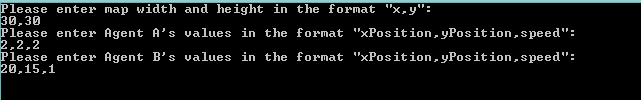
\includegraphics[width=1\textwidth]{Screenshots/StartingScreen}
  \caption{The information input screen.}
\end{figure}

\begin{figure}[h!]
  \centering
    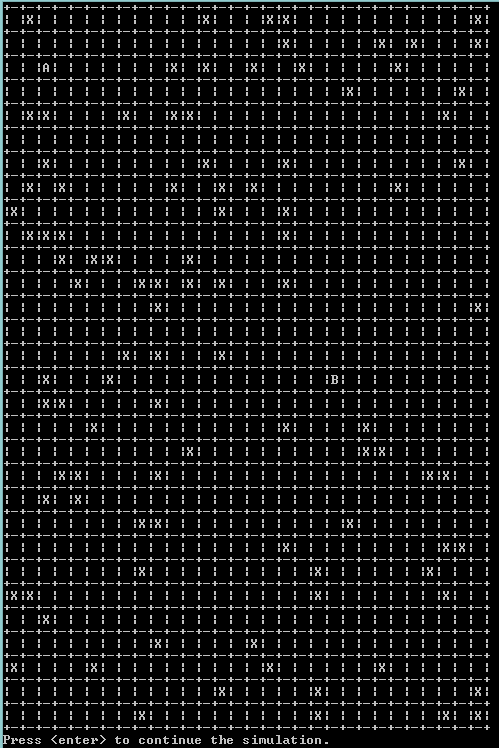
\includegraphics[width=0.8\textwidth]{Screenshots/Map}
  \caption{Starting screen based on the given information.}
\end{figure}
\clearpage